\section*{Figures}

%Figures should be uploaded as a separate file (or files) as .jpg or .tif files.

%Full instructions on preparing the figures are available as part of the online submission instructions. Please follow these instructions carefully as failure to do so will delay publication of your manuscript (please note: the editors reserve the right to charge for extensive changes).
%In preparing graphs authors should avoid background tints and 3D effects and maintain a consistent label size and aspect ratio (the x/y axis ratio) throughout a paper. Figure and axes titles should be clear and NOT in bold text. Do not include more figures than is absolutely necessary - non-essential figures may be judged as being suitable for online-only publication.

\begin{figure}[ht]
\centering
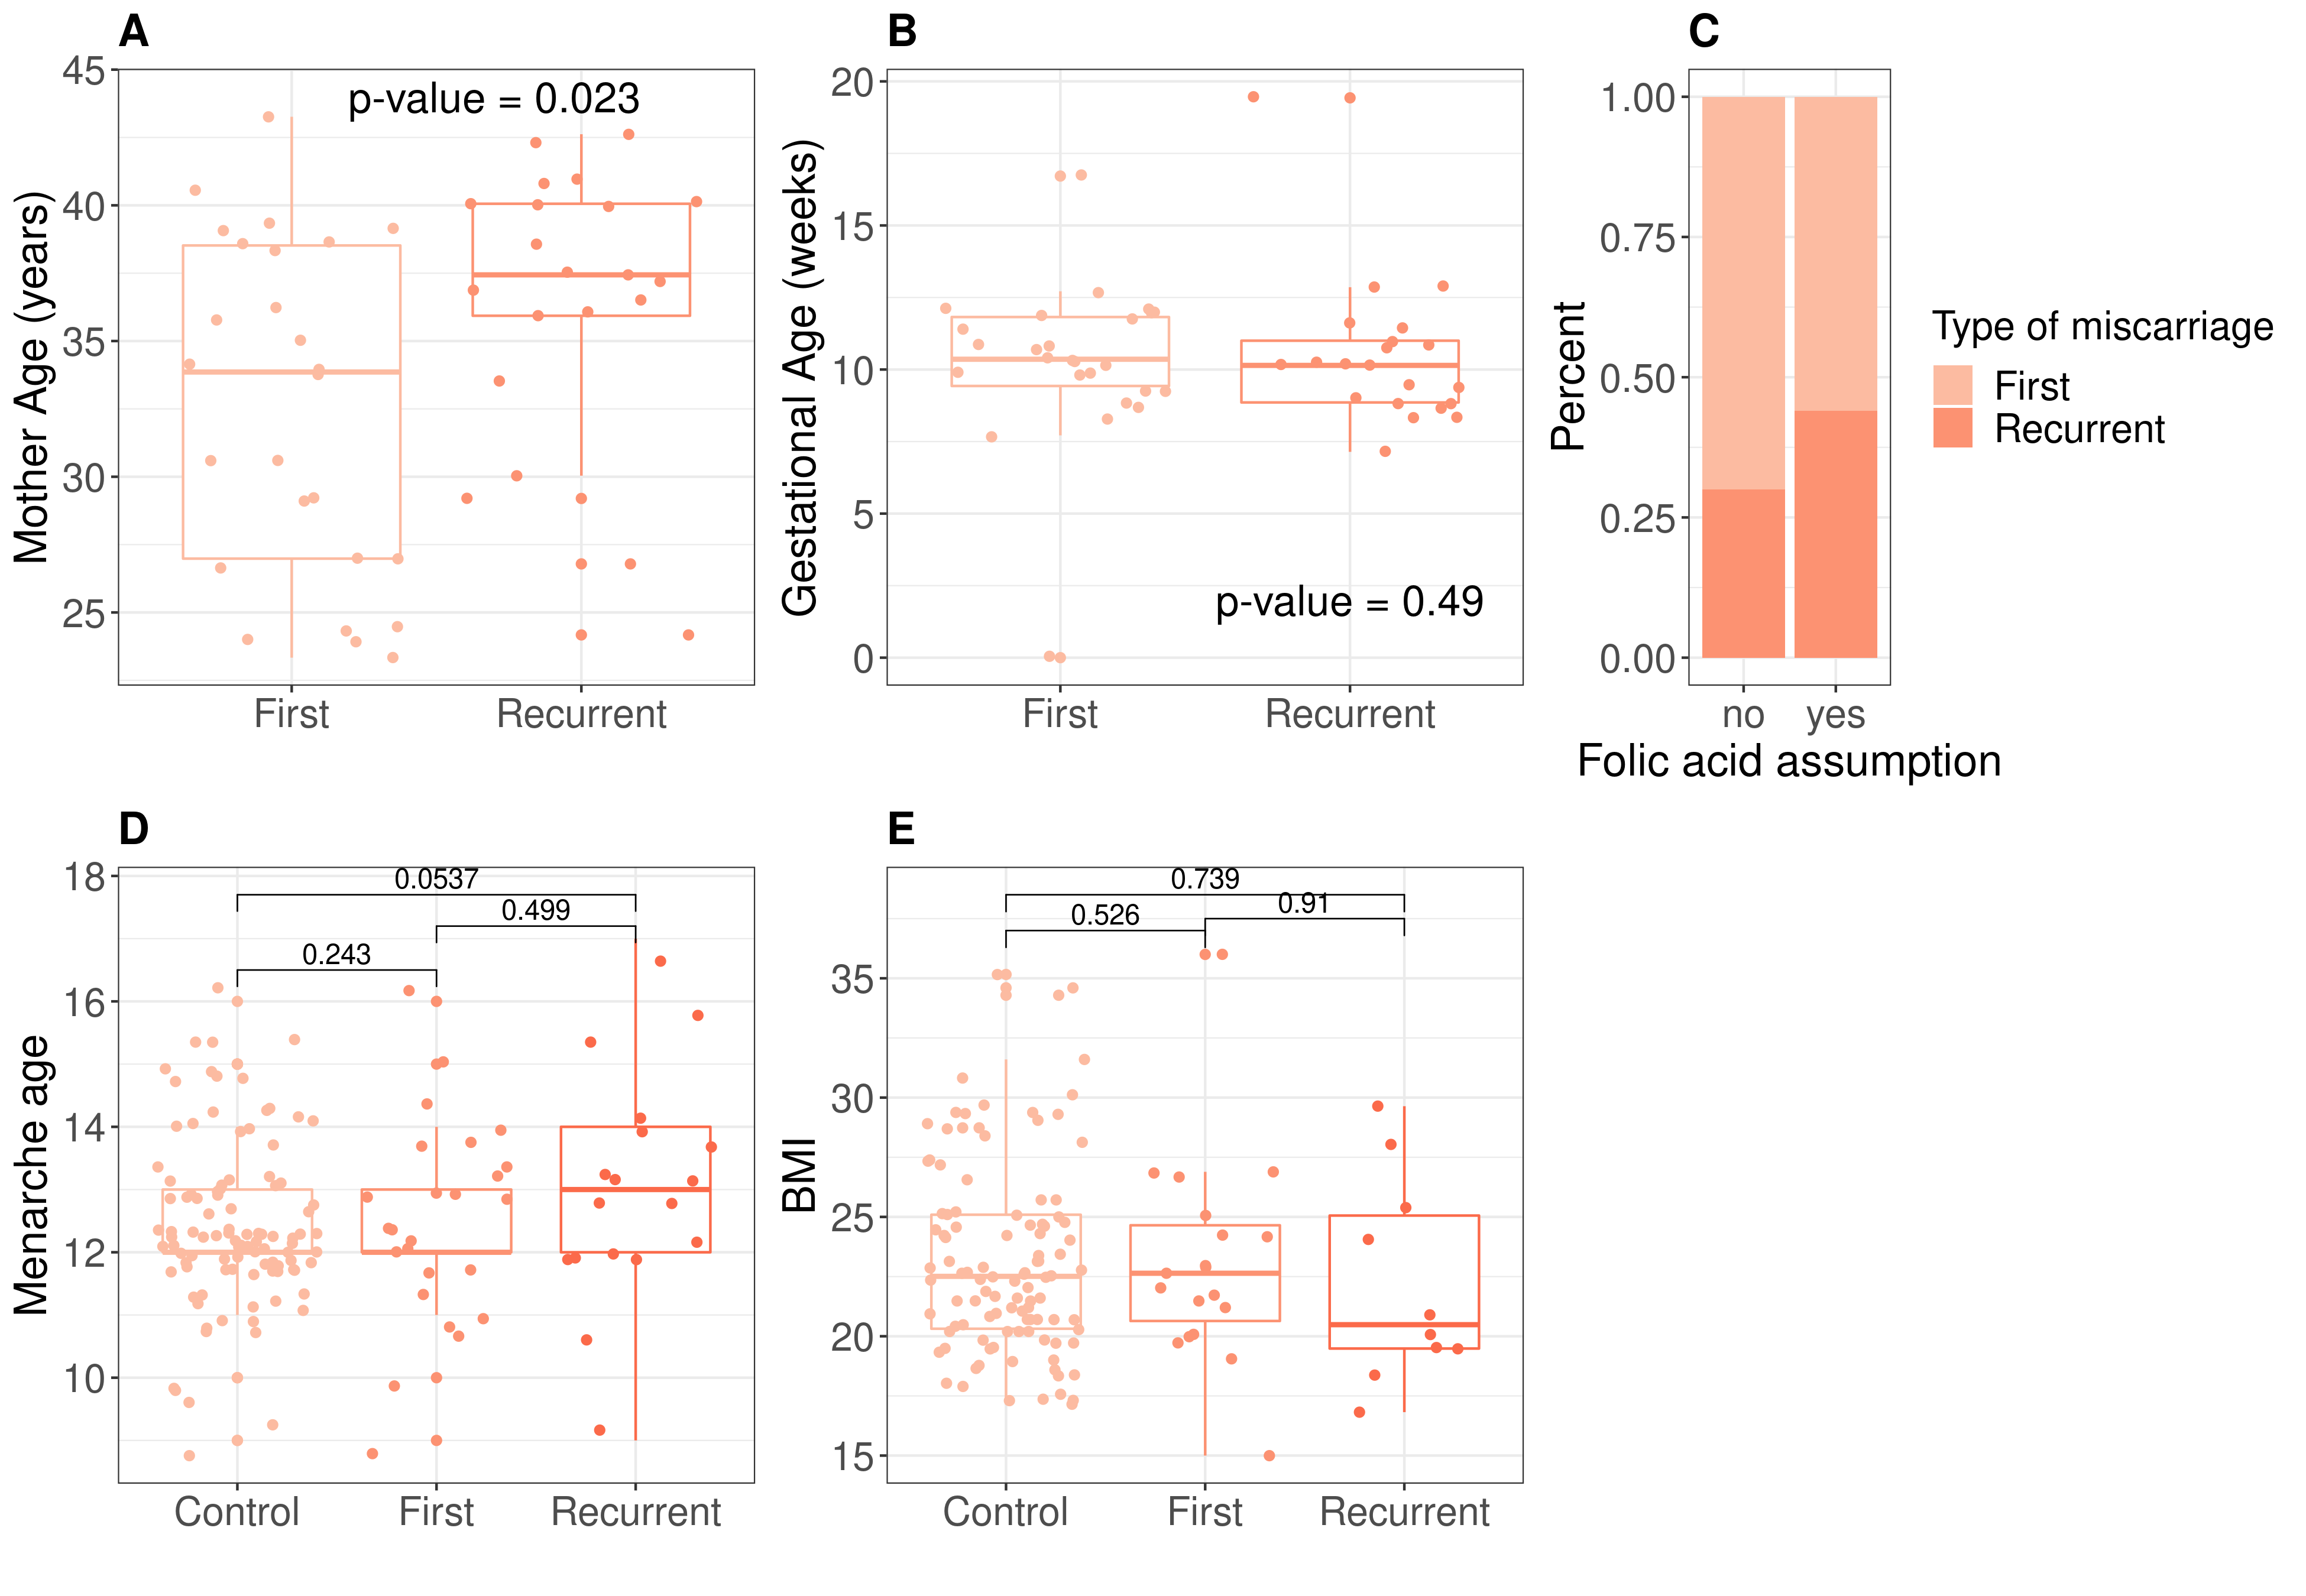
\includegraphics[width=\linewidth]{fig/panel_stats.png}
\caption{\textbf{Features of the embryo's mothers.} \textbf{(A)} Median age of the mother at the event is XX and XX for first and recurrent miscarriages, with no significant difference. \textbf{(B)} Gestational age at the time of the pregnancy termination range from X to X weeks with no significant difference between first and recurrent cases.  \textbf{(C)} Folic acid intake. Range of values of menarche age \textbf{(D)} and Body Mass Index \textbf{(E)} in embryo's mothers are not significantly different from a control set of mothers undergoing voluntary termination of pregnancy.}
\label{fig:embryostats}
\end{figure}

\begin{figure}[h]
\centering
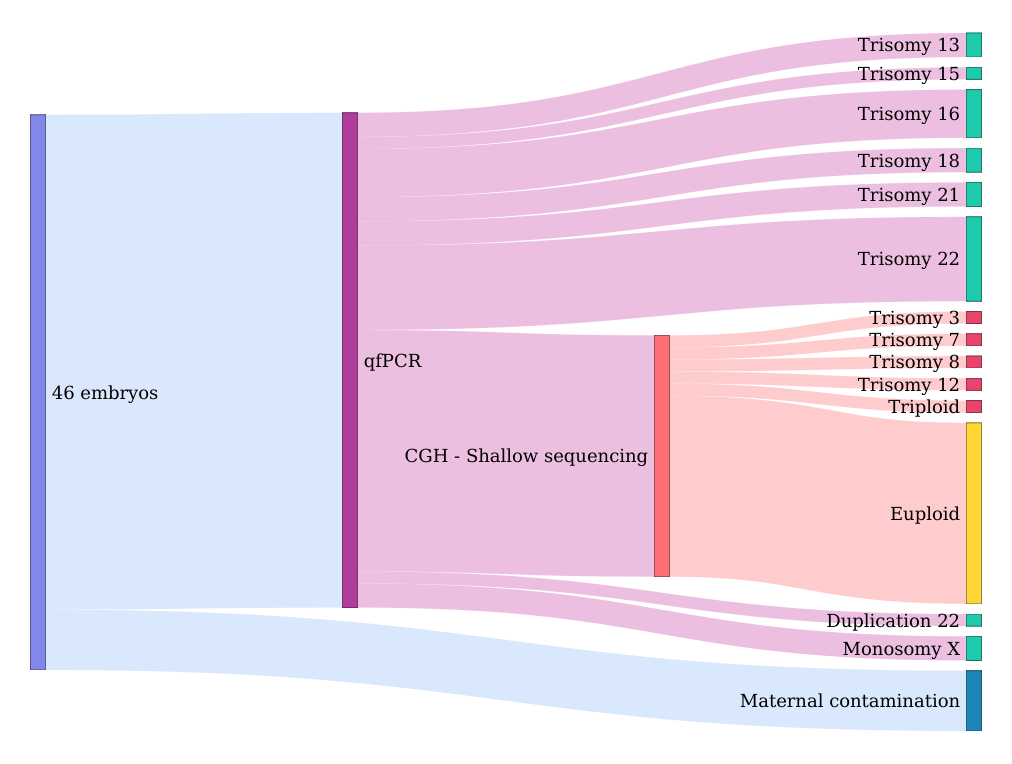
\includegraphics[width=0.7\textwidth]{fig/ibelieve.png}
\caption{\textbf{Outcome of the screening for aneuploidies in the embryos.} Screening on embryonic DNA by quantitative PCR, comparative hybridization and shallow sequencing finds aneuploidies in  56.6\% of the embryos, the most common being the trisomy of chromosome 22. In yellow the fraction of euploid embryos. }
\label{fig:presequencing}
\end{figure}

\begin{figure}[ht]
\centering
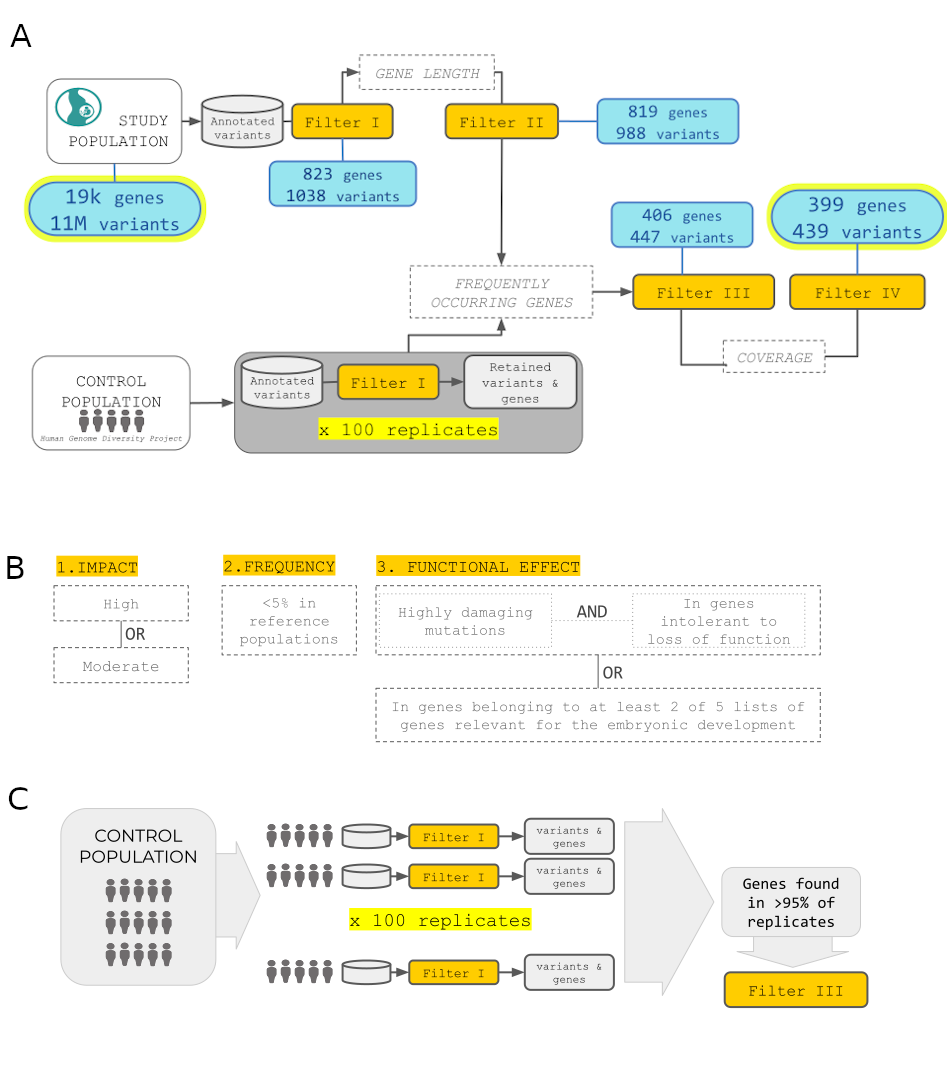
\includegraphics[width=\linewidth]{fig/pipe.png}
\caption{\textbf{Overview of the pipeline for prioritization of the genetic variants.} more text here } 
\label{fig:pipeline}
\end{figure}
%Genetic variants discovered in samples and controls are annotated and Filtered on the basis of the annotations (Filter I). In samples  Samples are first screened for the quality of DNA and maternal contamination and then analyzed for aneuploidies. \textbf{(B) Outcomes of the pipeline.} We estimate that 18\% of samples goes to sequencing....


\begin{figure}[ht]
\centering
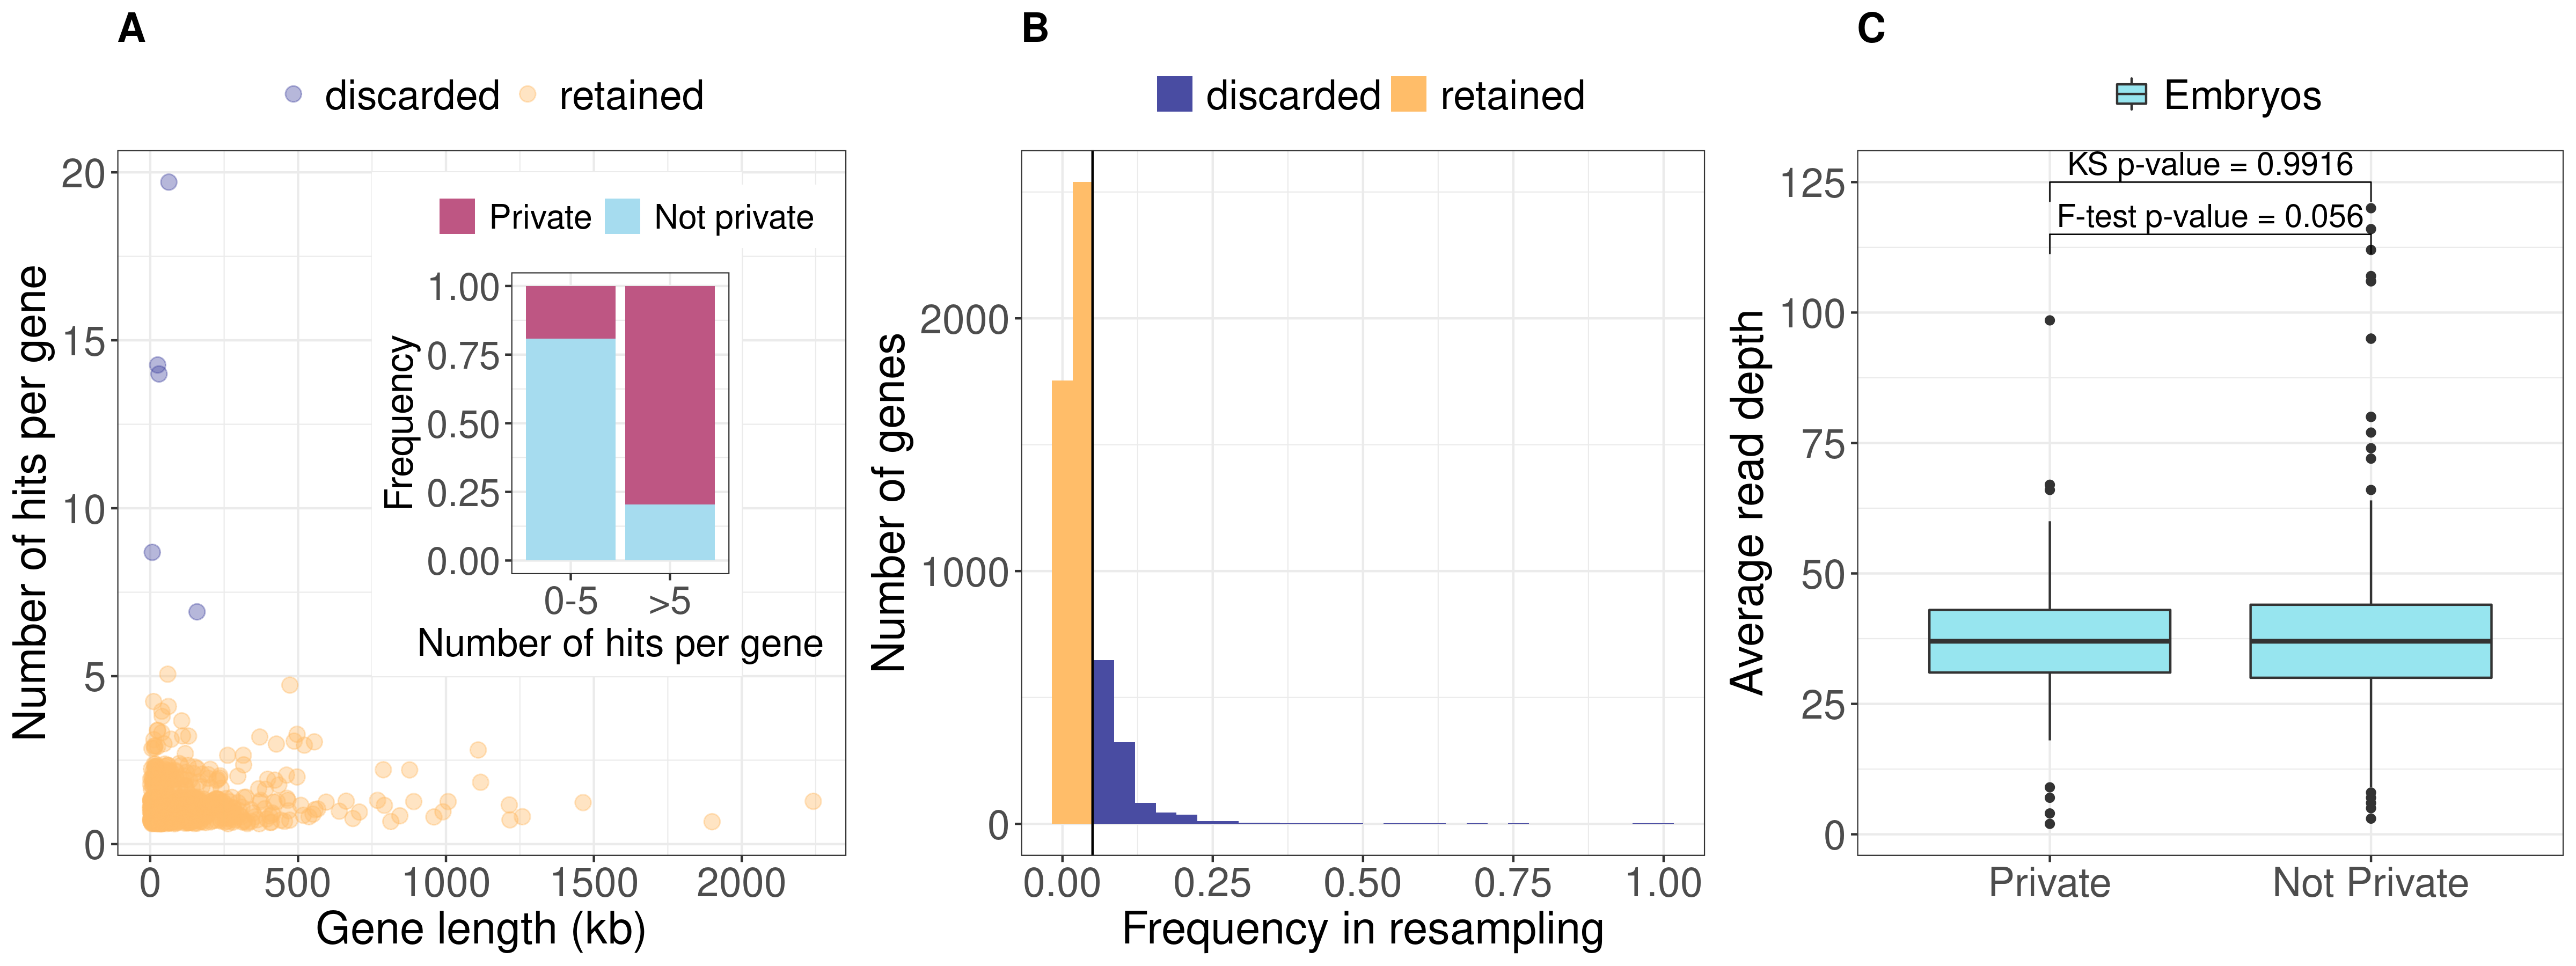
\includegraphics[width=\linewidth]{fig/filters_embryos.png}
\caption{\textbf{}}
\label{fig:filters}
\end{figure}

\begin{figure}[ht]
\centering
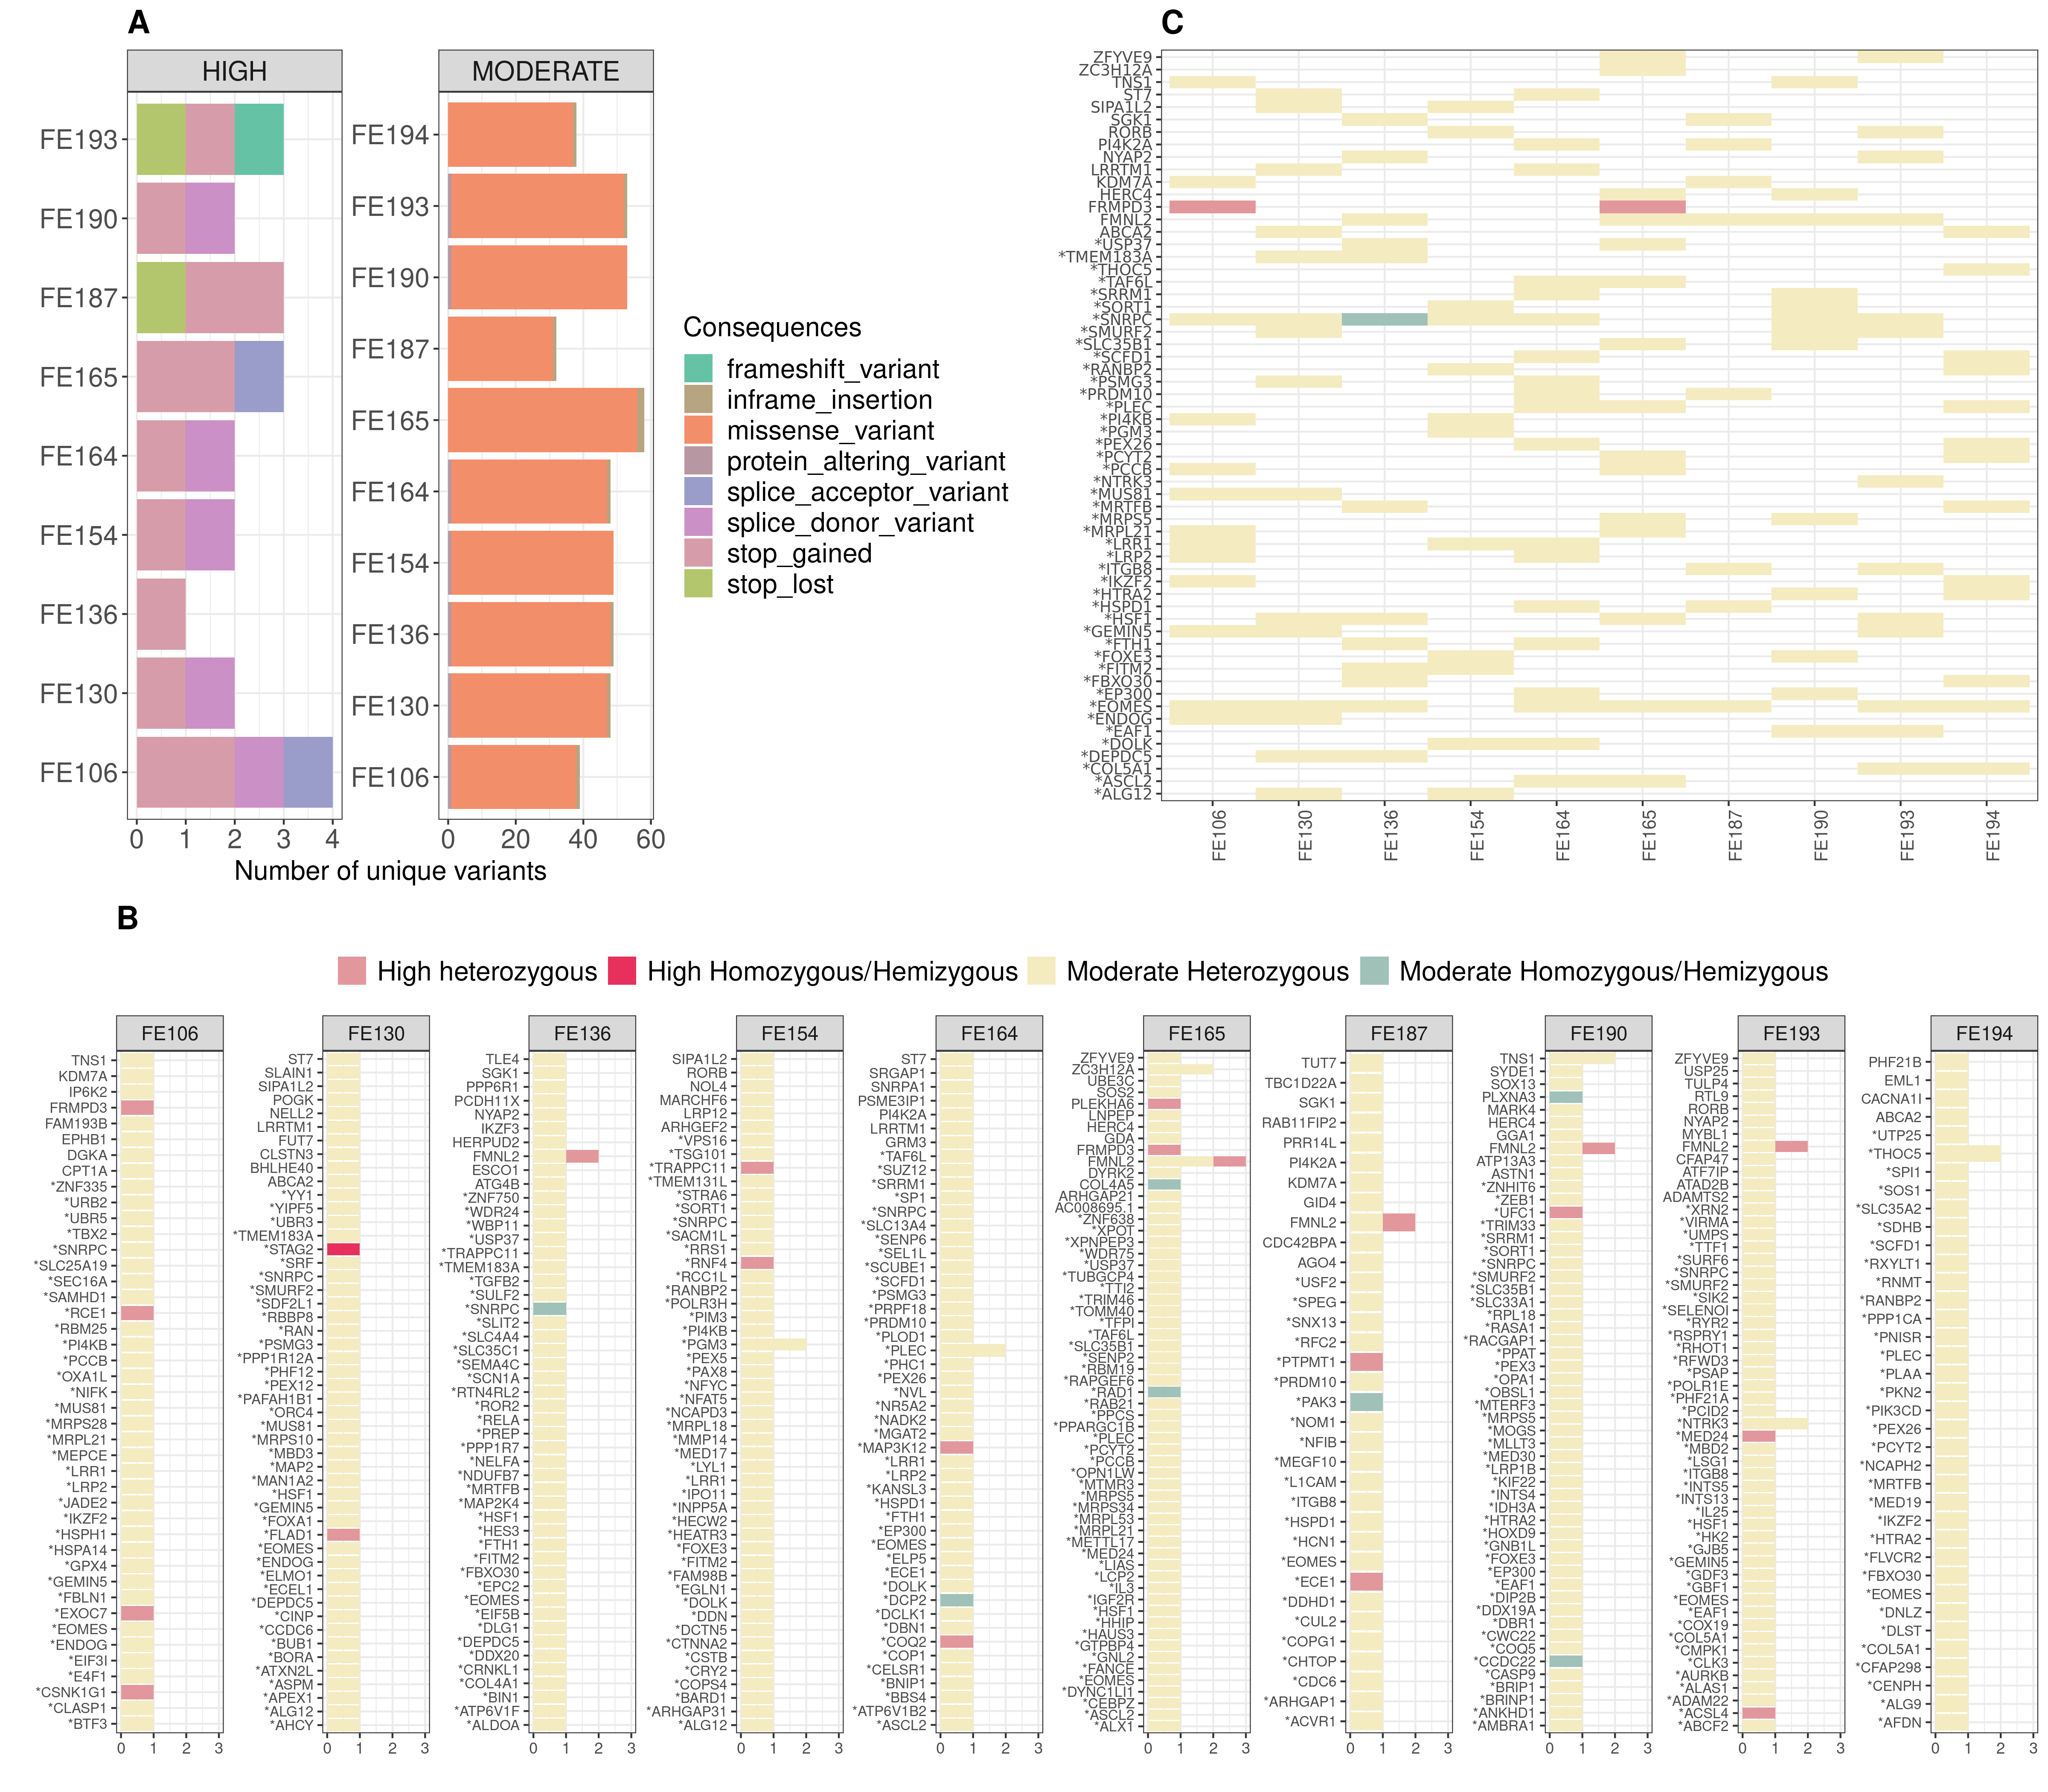
\includegraphics[width=\linewidth]{fig/panel_EmbryoResults.png}
%\caption{\textbf{} he occurrence of variants, their impact, and the count of the consequence allele per gene per embryo  }
\caption{\textbf{}}
\label{fig:resembryo}
\end{figure}

\begin{figure}[ht]
\centering
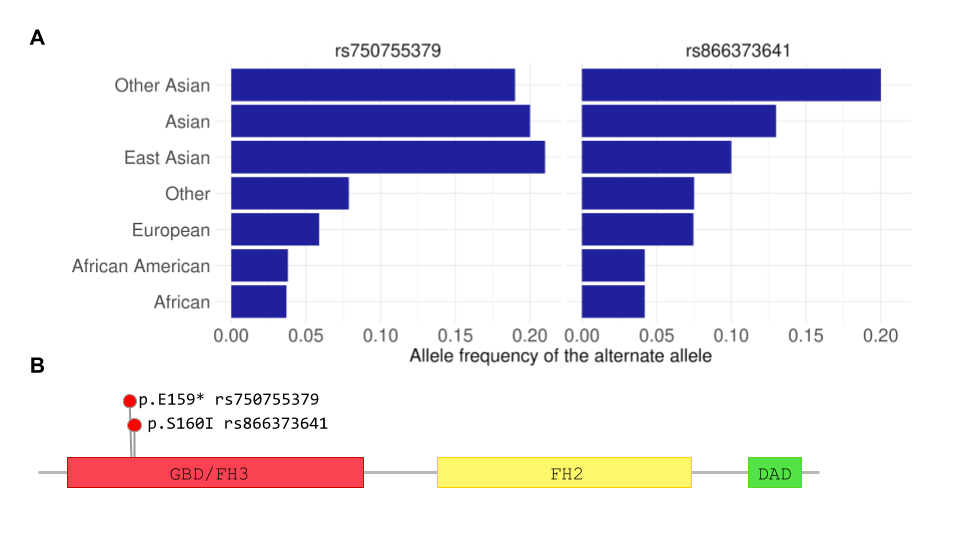
\includegraphics[width=\linewidth]{fig/fmnl2.png}
%\caption{\textbf{} he occurrence of variants, their impact, and the count of the consequence allele per gene per embryo  }
\caption{\textbf{}}
\label{fig:fmnl2}
\end{figure}